\pdfoutput=1
\documentclass[12pt,a4paper]{article}
\usepackage[utf8]{inputenc}
\usepackage{amsmath}
\usepackage{amsfonts}
\usepackage{amssymb}
\usepackage{amsthm}
\usepackage{graphicx}
\usepackage{todonotes}
\usepackage{natbib}
\usepackage{url}
\usepackage[boxruled,vlined,linesnumbered]{algorithm2e}
\usepackage{caption}
\usepackage{subcaption}
\usepackage{lineno}
\usepackage{tcolorbox}
\usepackage{caption}
\usepackage{hyperref}
\AtBeginDocument{\let\textlabel\label}
\hypersetup{colorlinks=true,linkcolor=black,citecolor=black,filecolor=black,urlcolor=black}

\captionsetup[figure]{labelfont=it,textfont={it},textfont=footnotesize}
\captionsetup[subfigure]{width=0.8\hsize,labelfont=bf,textfont=footnotesize,singlelinecheck=off,justification=raggedright,format=hang}

\theoremstyle{definition}
\newtheorem{definition}{Definition}



\author{Jonathan Rosenblatt \\ Ben Gurion University, 
	\and Roee Gilron \\ Tel Aviv University,
	\and Roy Mukamel \\ Tel Aviv University.}


%% OPTIONAL MACRO DEFINITIONS
%\def\s{\sigma}
\newcommand{\set}[1]{\{ #1 \}} % A set
\newcommand{\indicator}[1]{\mathcal{I}{\set{#1}}} % The indicator function.
\newcommand{\reals}{\mathbb{R}} % the set of real numbers
\newcommand{\features}{x} % The feature space
\newcommand{\outcomes}{y} % The feature space
\newcommand{\featureS}{\mathcal{X}} % The feature space
\newcommand{\outcomeS}{\mathcal{Y}} % The feature space
\newcommand{\expect}[1]{\mathbf{E}\left[ #1 \right]} % The expectation operator
\newcommand{\acc}{\mathcal{E}} 
\newcommand{\accEstim}{\hat{\mathcal{E}}} 
\newcommand{\accZ}{\hat{\mathcal{Z}}} 
\newcommand{\hyp}{\algo_{\data}(\features)} % A hypothesis
\newcommand{\hypFun}[2]{\algo_{#1}(#2)} % A hypothesis
\newcommand{\hypEstim}{\algo(\data)} %{\hat{\hyp}} % A hypothesis
\newcommand{\hypclass}{\mathcal{F}}
\newcommand{\prob}[1]{Prob( #1 )} % the probability of an event
\newcommand{\rv}[1]{\mathbf{#1}} % A random variable
\newcommand{\x}{\rv x} % The random variable x 
\newcommand{\y}{\rv y} % The random variable x 
\newcommand{\X}{\rv X} % The random variable x 
\newcommand{\Y}{\rv Y} % The random variable y
\newcommand{\gauss}[1]{\mathcal{N}\left(#1\right)} % The Gaussian distribution
\newcommand{\gaussp}[2]{\mathcal{N}_{#1}\left(#2\right)} % The Gaussian distribution
\newcommand{\mycaption}{Simulation details in Appendix~\ref{apx:simulation_details} except the changes in the sub-captions.}
\newcommand{\argmin}[2]{\mathop{argmin} _{#1}\set{#2}} % The argmin operator
\newcommand{\argmax}[2]{\mathop{argmax} _{#1}\set{#2}} % The argmin operator
\newcommand{\R}{\textsf{R }}
\newcommand{\algo}{\mathcal{A}}
\newcommand{\data}{\mathcal{S}}
\newcommand{\measure}{\mathcal{P}}
\newcommand{\measuren}{\measure^n}
\newcommand{\union}{\cup}
\newcommand{\intersect}{\cap}
\newcommand{\majority}{\accEstim_{Maj}}


\title{Better-Than-Chance Classification for Signal Detection}


\begin{document}
%Sketch: 
%- The conservativeness of the test. 
%- What does it detect?
%- Is it remedied in large samples?
%- Is conservativeness always there?


\maketitle
%\linenumbers

\begin{abstract}
We show that using a classifier's accuracy as a test statistic, is underpowered for the purpose of finding a difference between populations, compared to a bona-fide statistical test.
It is also more complicated to implement, so that a statistical test should be preferred. 
For the cases that the goal of the test is not the existence of a difference between populations, but the actual classification ability, we suggest several improvements to the classification accuracy, to increase its power against a ``pure chance'' null. 
\end{abstract}


%%%% Introduction %%%
\section{Introduction}
\label{sec:introduction}

A common workflow in neuroimaging consists of fitting a classifier, and estimating its predictive accuracy using cross validation. 
Given that the cross validated accuracy is a random quantity, it is then common to test if the cross validated accuracy is significantly better than chance using a permutation test.  
Examples in the neuroscientific literature include \citet{golland_permutation_2003,pereira_machine_2009,varoquaux_assessing_2016}, and especially the recently popularized \emph{multivariate pattern analysis} (MVPA) framework of \citet{kriegeskorte_information-based_2006}.
This practice is also observed in some high profile publications in the genetics literature: 
\citet{golub_molecular_1999,slonim_class_2000,radmacher_paradigm_2002,mukherjee_estimating_2003,juan_prediction_2004,jiang_calculating_2008}.


To fix ideas, we will adhere to a concrete example.
In \cite{gilron_quantifying_2016}, the authors seek to detect brain regions which encode differences between vocal and non-vocal stimuli. 
Following the MVPA workflow, the localization problem is cast as a supervised learning problem: if the type of the stimulus can be predicted from the spatial activation pattern significantly better than chance, then a region is declared to encode vocal/non-vocal information. 
We call this an \emph{accuracy test}, a.k.a.\ \emph{class prediction}, or \emph{pattern discrimination} 

This same signal detection task can be also approached as a two-group multivariate test.
Inferring that a region encodes vocal/non-vocal information, is essentially inferring that the spatial distribution of brain activations is different given a vocal/non-vocal stimulus. 
As put in \cite{pereira_machine_2009}: 
\begin{quote}
... the problem of deciding whether the classifier learned to discriminate the classes can be subsumed into the more general question as to whether there is evidence that the underlying distributions of each class are equal or not.
\end{quote}
A practitioner may thus approach the signal detection problem with a two-group population test such as Hotelling's $T^2$ \citep{anderson_introduction_2003}.
Alternatively, if the size of brain region of interest is large compared to the number of observations, so that the spatial covariance cannot be fully estimated, then a high dimensional version of Hotelling's test can be called upon, such as in \cite{schafer_shrinkage_2005} or \cite{srivastava_multivariate_2007}.
For brevity, and in contrast to \emph{accuracy tests}, we will call any two-sample multivariate tests simply \emph{population tests}, a.k.a.\ \emph{class comparisons}. 
%TODO: rename population test to parameter test?


At this point, it becomes unclear which is preferable: a population test or an accuracy test?
The former with a heritage dating back to \cite{hotelling_generalization_1931}, and the latter being extremely popular, as the $959$ citations\footnote{GoogleScholar. Accessed on Aug 4, 2016.} of \cite{kriegeskorte_information-based_2006} suggest. 

The comparison between population and accuracy tests was precisely the goal of \cite{ramdas_classification_2016}, who compared the $T^2$ population test to the accuracy of \emph{Fisher's linear discriminant analysis} classifier (LDA). 
By comparing the rates of convergence of the powers to $1$, \cite{ramdas_classification_2016} concluded that accuracy and population tests are rate equivalent. 

Asymptotic relative efficiency measures (ARE) are typically used by statisticians to compare between rate-equivalent test statistics \citep{vaart_asymptotic_1998}.
\cite{ramdas_classification_2016} derive the asymptotic power functions of the two test statistics, which allows to compute the ARE between Hotelling's $T^2$ (population) test and Fisher's LDA (accuracy) test.
Theorem~14.7 of \cite{vaart_asymptotic_1998} relates asymptotic power functions to ARE.
Using this theorem and the results of \cite{ramdas_classification_2016} we deduce that the ARE is lower bounded by $2 \pi \approx 6.3$. 
This means that Fisher's LDA requires at least $6.3$ more samples to achieve the same (asymptotic) power than the $T^2$ test. 
In this light, the accuracy test is remarkably inefficient compared to the population test.  
For comparison, the t-test is only $1.04$ more (asymptotically) efficient than Wilcoxon's rank-sum test \citep{lehmann_parametric_2009}, so that an ARE of $6.3$ is strong evidence in favor of the population test. 

Before discarding accuracy tests as inefficient, we recall that \cite{ramdas_classification_2016} analyzed a \emph{half-sample} holdout. 
The authors conjectured that a leave-one-out approach, which makes more efficient use of the data, may have better performance. 
Also, the analysis in \cite{ramdas_classification_2016} is asymptotic. 
This eschews the discrete nature of the accuracy statistic, which will be shown to have  crucial impact. 
Since typical sample sizes in neuroscience are not large, we seek to study which test is to be preferred in finite samples? 
Our conclusion will be quite simple: {\em population tests typically have more power than accuracy tests, and are easier to implement.}

Our statement rests upon the observation that with typical sample sizes, the accuracy test statistic is highly discrete. 
Permutation testing with discrete test statistics are known to be conservative \citep{hemerik_exact_2014}, since they are insensitive to mild perturbations of the data, and they cannot exhaust the permissible false positive rate. 
As simply put by Frank Harrell in \textsf{CrossValidated\footnote{A Q\&A website for statistical questions: \url{http://stats.stackexchange.com/questions/17408/how-to-assess-statistical-significance-of-the-accuracy-of-a-classifier}}} post back in $2011$:
\begin{quote}
	... your use of proportion classified correctly as your accuracy score. This is a discontinuous improper scoring rule that can be easily manipulated because it is arbitrary and insensitive.
\end{quote}


The degree of discretization is governed by the number of samples. 
In our example from \citet{gilron_quantifying_2016}, the classification is computed using $40$ examples, so that the test statistic may assume only $40$ possible values. 
This number of examples is not unusual if considering this is the number of trial-repeats, or the number of subjects, in an neuroimaging study. 

The discretization effect is aggravated if the test statistic is highly concentrated. 
For an intuition consider the usage of a the \emph{resubstitution accuracy} as a test statistic. 
This statistic simply means that the accuracy is not cross validated, but rather evaluated on the training data.
If the data is high dimensional, the resubstitution accuracy will be very high due to over fitting. 
In a very high dimensional regime, the resubstitution accuracy will be $1$ for the observed data \cite[Theorem 1]{mclachlan_bias_1976}, but also for any permutation.
The concentration of resubstitution accuracy near $1$, and its discreteness, render this test completely useless, with power tending to $0$ for any (fixed) effect size, as the dimension of the model grows. 


To compare the power of accuracy tests and population tests in finite samples, we study a battery of test statistics by means of simulation. 
We start with formalizing the problem in Section~\ref{sec:problem_setup}.
The main findings are reported in Sections~\ref{sec:power}, \ref{sec:example} and Appendix~\ref{apx:simulations}.
A discussion follows in Section~\ref{sec:discussion}. 



%%%% Section %%%%
\section{Problem setup}
\label{sec:problem_setup}

Let $\outcomes \in \outcomeS$ be a class encoding. 
Let $\features \in \featureS$ be a $p$ dimensional feature vector. 
In our vocal/non-vocal example we have $\outcomeS=\set{-1,1}$ and $p$, the number of voxels in a brain region so that $\featureS=\reals^{27}$. 

Given $n$ pairs of $(\features_i,\outcomes_i)$, typically assumed i.i.d., a population test amounts to testing whether $\features|\outcomes=1$ has the the same distribution as $\features|\outcomes=-1$. 
I.e., we test if the multivariate voxel activation pattern has the same distribution when given a vocal stimulus, as when given a non-vocal stimulus. 

An accuracy test amounts to learning a predictive model and testing if its predictions $y|x$ are better than chance. 
Denoting a dataset by $\data:=(\features_i,\outcomes_i)_{i=1}^n$, the a predictor, $\hyp:\featureS \to \outcomeS$, is the output of a learning algorithm $\algo$ when applied to the dataset $\data$, so that $\algo:\data \to \hyp$. 
The accuracy of predictor, $\acc_{\hyp}$, is defined as the probability of $\hyp$ making a correct prediction.
The accuracy of an algorithm, $\acc_{\algo}$, is defined as the expected accuracy over all possible data sets. 
Formally-- denoting by $\measure$ the probability measure of $(\features, \outcomes)$, and by $\measuren$ the same for the i.i.d sample $\data$, then
\begin{align}
	\acc_{\hyp}:=\int_{(\features,\outcomes)} \indicator{\hyp=\outcomes} \; d\measure(\features,\outcomes),
\end{align}
and
\begin{align}
	\acc_{\algo}:=\int_\data \acc_{\algo_\data} \; d\measuren(\data).
\end{align}
Denoting an estimate of $\acc_{\hyp}$ by $\accEstim_{\hyp}$, and $\acc_{\algo}$ by $\accEstim_{\algo}$, 
a statistically significant ``better than chance'' estimate of either,  is evidence that the classes are distinct. 
In a typical application, the predictor is not fixed, so that $\accEstim_{\algo}$, and not $\accEstim_{\hyp}$, will be used for the testing. 

Two popular estimates of $\accEstim_{\algo}$ are the \emph{resubstitution estimate}, and the V-fold cross validation (CV) estimate.
\begin{definition}[Resubstitution estimate]
\label{def:resubstitution}
The resubstitution accuracy estimator, $\accEstim_{\algo}^{Resub}$,  is defined as
\begin{align}
	\accEstim_{\algo}^{Resub} := \frac 1n \sum_{i=1}^{n} \indicator{\hypFun{\data}{\features_i}=\outcomes_i}, 
\end{align}
where $\indicator{A}$ is the indicator function of event $A$. 
\end{definition}


\begin{definition}[V-fold CV estimate]
\label{def:v-fold}
Denoting by $\data^{v}$ the $v$'th partition, or \emph{fold}, of the dataset, and by $\data^{(v)}$ its complement, so that $\data^{v} \union \data^{(v)}=\union_{v=1}^V \data^{v}=\data$, the V-fold CV accuracy estimator, $\accEstim_{\algo}^{Vfold}$, is defined as 	
\begin{align}
	\accEstim_{\algo}^{Vfold} := 
	\frac 1V \sum_{v=1}^{V} \frac{1}{|\data^v|} \sum_{i \in \data^{v}} \indicator{\hypFun{\data^{(v)}}{\features_i}=\outcomes_i}, 
\end{align}
\end{definition}




\subsection{Candidate Tests}
\label{sec:considerations}

The design of a permutation test using $\accEstim_{\algo}$ requires the following design choices: 
\begin{enumerate}
\item Is $\accEstim_{\algo}$ cross validated or not?
\item For a V-fold cross validated test statistic:
\begin{enumerate}
\item Should the data be refolded in each permutation? 
\item Should the data folding be balanced (a.k.a.\ stratified)?
\item How many folds? 
\end{enumerate}
\item How to estimate $\accEstim_{\algo}$?
\end{enumerate}

We will now address these questions while bearing in mind that unlike the typical supervised learning setup, we are not interested in an unbiased estimate of $\acc_{\algo}$, but rather in the detection of its departure from chance level. 

\paragraph{Cross validate or not?}
Given our goal, a biased estimate of $\accEstim_{\algo}$ is not a problem provided that bias is consistent over all permutations. 
The underlying intuition is that a permutation test will be unbiased, provided that the exact same computation is performed over all permutations. 
We will thus be considering both cross validated accuracies, and resubstitution accuracies.


\paragraph{Balanced folding?}
The standard practice when cross validating is to constrain the data folds to be balanced, i.e. stratified \citep[e.g.][]{ojala_permutation_2010}.
This means that each fold has the same number of examples from each class. 
We will report results with both balanced and unbalanced data foldings, only to discover, it does not seem to matter. 


\paragraph{Refolding?}
The standard practice in neuroimaging is to permute labels and refold the data after each permutation, so that the balance of the classes in each fold is preserved.
We will adhere to this practice due to its popularity, even though it can be avoided by permuting features instead of labels, as done by \citet{golland_permutation_2005}.


\paragraph{How many folds?}
Different authors suggest different rules for the number of folds. 
We will look into the effect of the number of folds. 

\paragraph{How to estimate accuracy?}
\label{sec:estimate_accuracy}
Lower than $0.5$ accuracies, known as \emph{anti-learning}, are evidence that signal is present and classes are separated. Given out detection purposes, we should consider the departure from chance level $|\accEstim_{\algo}-0.5|$ as candidate test statistic.
For unbalanced classes, chance level is not $0.5$, but rather the the probability of the majority class, which we denote by $\majority$.
This suggests the following test statistic $|\accEstim_{\algo}-\majority|$.
Since we will be aggregating these statistics over random data sets where $\majority$ may vary, it seems appropriate to standardize the scale. 
We thus study, along with the naive accuracy estimate, $\accEstim_{\algo}$ , also the \emph{z-scored accuracy} of algorithm $\algo$:
\begin{align}
\label{eq:z_scored_accuracy}
	\accZ_{\algo} := \frac{|\accEstim_{\algo}-\majority|}{\sqrt{\majority(1-\majority)}}.
\end{align} 

\bigskip

Table~\ref{tab:collected} collects an initial battery of tests we will be comparing. 
\begin{tcolorbox}
\centering
\begin{tabular}{l|c|c|c|c}
Name & Algorithm & Accuracy & Z-scored & Parameters\\ 
\hline
\hline
Hotelling & Hotelling & -- & -- & -- \\ 
Hotelling.shrink & Hotelling & -- & -- & -- \\ 
sd & Hotelling & -- & -- & -- \\ 
lda.CV.1 	& LDA & V-fold 			& FALSE 	&  -- \\ 
lda.CV.2 	& LDA & V-fold 			& TRUE 	& -- \\ 
lda.noCV.1 	& LDA & Resubstitution 	& FALSE 	&  --\\ 
lda.noCV.2 	& LDA & Resubstitution 	& TRUE 	&  --\\ 
svm.CV.1 	& SVM & V-fold 			& FALSE & cost=$10$ \\ 
svm.CV.2 	& SVM & V-fold 			& FALSE & cost=$0.1$ \\ 
svm.CV.3 	& SVM & V-fold 			& TRUE 	& cost=$10$ \\ 
svm.CV.4 	& SVM & V-fold 			& TRUE 	& cost=$0.1$ \\ 
svm.noCV.1 	& SVM & Resubstitution 	& FALSE & cost=$10$ \\ 
svm.noCV.2 	& SVM & Resubstitution 	& FALSE & cost=$0.1$ \\ 
svm.noCV.3 	& SVM & Resubstitution 	& TRUE 	& cost=$10$ \\ 
svm.noCV.4 	& SVM & Resubstitution 	& TRUE 	& cost=$0.1$ \\
\end{tabular} 
\captionsetup{type=table}
\caption{\footnotesize
This table collects the various test statistics we will be studying. 
Three are population tests: \emph{Hotelling}, \emph{Hotelling.shrink}, and \emph{sd}.
\textit{Hotelling} is the classical two-group $T^2$ statistic. 
\textit{Hotelling.shrink} is a high dimensional version with the regularized covariance from \citet{schafer_shrinkage_2005}. 
\textit{sd} is another high dimensional version of the $T^2$, from \citet{srivastava_two_2013}.
The rest of the tests are variations of the linear SVM, and Fisher's LDA, with varying accuracy measures, cross validated or not, and varying tuning parameters. 
For example, \textit{svm.CV.4} is a linear SVM (implemented with the \emph{svm} \R function \citep{meyer_e1071:_2015}),
the cost parameter set at $0.1$, and using the cross validated z-scored accuracy in Eq.~\ref{eq:z_scored_accuracy}.
Another example is \textit{lda.noCV.1}, which is Fisher's LDA, returning the resubstitution accuracy.}
\label{tab:collected}
\end{tcolorbox}







%%%% Section %%%%
\section{Controlling the False Positive Rate}
\label{sec:type_i}

Our simulations show that all of the tests considered conserve the desired $0.05$ false positive rate, up to varying levels of conservatism.
This can be seen from the fact that the probability of rejection is no higher than $0.05$ in the absence of any effect, encoded by a red circle. 
This is true, in particular if: \newline
(a) The folds are balanced or not (Figures~\ref{fig:simulation_1},\ref{fig:n_folds} and \ref{fig:n_folds_unbalanced}). \newline
(b) The tuning parameters are varied (cost=$10$ versus cost=$0.1$). \newline
(c) The number of folds is varied (Figures \ref{fig:n_folds} and \ref{fig:n_folds_unbalanced}). \newline
(d) The noise is heavytailed (Figure~\ref{fig:t_null}). \newline
(e) The problem is high or low dimensional (Figure~\ref{fig:large_sample}.) \newline
(f) The noise is correlated (Figure~\ref{fig:ar_1}). \newline
We also observe that the most conservative tests are the resubstitution accuracy statistics. 
We return to this matter in the Discussion.







%%%% Section %%%%
\section{Power}
\label{sec:power}

Having established that all of the tests in our battery control the false positive rate, it remains to be seen if they have similar power-- 
especially when comparing population tests to accuracy tests. 
From the simulation results reported in Appendix~\ref{apx:simulations} we collect the following insights:
\begin{enumerate}
\item Population tests have no less-- and typically more-- power than accuracy tests in our simulations.

\item The conservativeness of accuracy tests decays as the sample grows (Figures~\ref{fig:large_sample_1}, \ref{fig:large_sample_2} and \ref{fig:large_sample_3})

\item For heavy tailed distributions (Figure~\ref{fig:t_null}), the difference in power between population tests and accuracy tests vanishes. 

\item Regularization is critical to power as can be seen by comparing \emph{Hotelling} to \emph{Hotelling.shrink} and \emph{sd}.

\item The z-scoring of the accuracies was introduced to deal with unbalanced foldings. 
If the z-scoring has any effect at all, it merely diminishes power.
The non-z-scored accuracy tests are unaffected by the balance of the folding.

\item Both accuracy and population tests are inappropriate for scale alternatives (Figure~\ref{fig:scale_change}). 
This was to be expected and is reported mostly as a sanity check (cost=10 vs. cost=0.1 statistics).

\item Balanced folding only affects the z-scored accuracy, in the opposite direction than we anticipated. 

\item Increasing the SVM's cost parameter, which reduces the number of support vectors entering the classifier, reduces power. 

\end{enumerate}


The major insight from simulations is that the use of accuracy tests for signal detection is underpowered compared to population tests. 
We have not established, however, that the dominance of the population tests is not due to their regularization. Indeed, the unregularized \emph{Hotelling} test, is only slightly superior to the accuracy tests. 
We return to this matter in Section~\ref{sec:highdim}, by adding some regularized accuracy tests to our battery. 
We now verify our finding on a neuroimaging dataset.



\section{Neuroimaging Example}
\label{sec:example}
% Power of SVM versus SD.
% Difficulties of implementation.

Figure~\ref{fig:read_data} is an application of both a population and an accuracy test to the data of \cite{pernet_human_2015}. 
The authors of \cite{pernet_human_2015} collected fMRI data while subjects were exposed to the sounds of human speech (vocal), and other non-vocal sounds. 
Each subject was exposed to $20$ sounds of each type, totaling in $n=40$ trials.
The study was rather large and consisted of about $200$ subjects.
The data was kindly made available by the authors at the OpenfMRI website\footnote{\url{https://openfmri.org/}}.

We perform group inference using within-subject permutations along the analysis pipeline of \cite{stelzer_statistical_2013}, which was also reported in \cite{gilron_quantifying_2016}. 
To demonstrate our point, we compare the \emph{sd} population test with the \emph{svm.cv.1} accuracy test. 

In agreement with our simulation results, the population test (\emph{sd}) discovers more brain regions of interest when compared to an accuracy test (\emph{svm.cv.1}).
The former discovers $1,232$ regions, while the latter only $441$, as depicted in Figure~\ref{fig:read_data}.
We emphasize that both test statistics were compared with the same permutation scheme, and the same error controls, so that any difference in detections is due to their different power.


\begin{figure}[th]
\centering
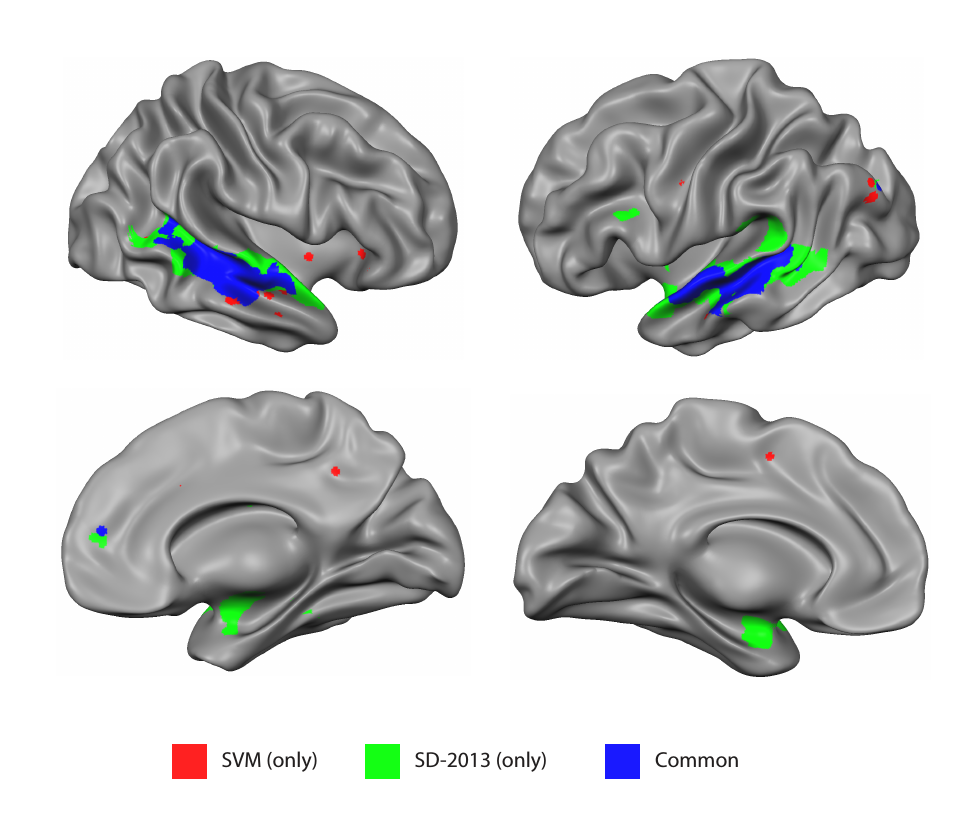
\includegraphics[width=0.7\linewidth]{art/svm_vs_SD}
\caption{\footnotesize
Brain regions encoding information discriminating between vocal and non-vocal stimuli.
Map reports the centers of $27$-voxel sized spherical regions, as discovered by an accuracy test (\emph{svm.cv.1}), and a population test (\emph{sd}). 
\emph{svm.cv.1} was computed using $5$-fold cross validation, and a cost parameter of $1$. 
Region-wise significance was determined using the permutation scheme of \cite{stelzer_statistical_2013}, followed by region-wise $FDR \leq 0.05$ control using the Benjamini-Hochberg procedure \citep{benjamini_controlling_1995}.
Number of permutations equals $400$.
The population test detect $1,232$ regions, and the accuracy test $441$, $399$ of which are common to both.
For the details of the analysis see \cite{gilron_quantifying_2016}.  
  }
\label{fig:read_data}
\end{figure}








%%%% Section %%%%
\section{Discussion}
\label{sec:discussion}

We have set out to understand which of the tests is more powerful: accuracy tests or population tests. 
No amount of simulations can replace the insight provided by a closed-form analytic result. 
The finite sample power of permutation tests is a formidable mathematical problem, so we currently content ourselves with simulations.
We have concluded that the population tests are typically preferable. 
Their high dimensional versions, such as \cite{srivastava_multivariate_2007} and \cite{schafer_shrinkage_2005},  are particularly well suited for neuroimaging problems such as MVPA.
We attribute this to several effects: \newline
(a) The discrete nature of the accuracy test in finite samples. \newline
(b) Inefficient use of the data when validating with a holdout set. \newline
(c) The lack of regularization in high SNR regimes (high dimension and\slash or strong correlations). \newline


The degree of discretization is governed by the sample size. 
For this reason, an asymptotic analysis such as \cite{ramdas_classification_2016} may uncover the holdout inefficiency, but will not uncover the discretization effect. 
An asymptotic analysis of a finite complexity model, such as \cite[Sec~4.3]{golland_permutation_2005}, would also fail to reveal the effect of the concentration of the resubstitution accuracy near $1$. This effect would render the resubstitution estimates a legitimate asymptotic test, and a terrible finite sample test. 

Simulations do show cases where population tests have no advantage over accuracy tests. 
One such scenario is when the noise is heavytailed, as seen in Figure~\ref{fig:t_null}.
The second scenario will be discussed in Section~\ref{sec:highdim}.

The practical advice for the practitioner, is that for the purpose of signal detection, there is typically a population test that is more powerful than an accuracy test. 
The class of population tests we examined, in particular their regularized versions, are good performers in a wide range of simulation setups and empirically. 
They are also typically easier to implement, and faster to run, since no cross validation will be involved. 



\subsection{Ease of implementation}
A very important consideration is the ease of implementation. 
The need for cross validation of the accuracy test greatly increases its computational complexity. 
Moreover, programming with discrete statistics is more prone to errors. 
This is because their unforgiveness to the type of inequalities used. 
Indeed, mistakenly replacing a weak inequality with a strong inequality in one's program may considerably change the results. 
This is not the case for continuous test statistics. 




\subsection{Reservations}
\label{sec:reservations}

Some reservations to the generality of our findings are in order. 
Firstly, not all accuracy tests are concerned with signal detection.
Consider brain decoding for machine interfaces, or clinical diagnosis, where the presence of a medical condition is predicted from imaging data \citep[e.g.][]{olivetti_induction_2012,wager_fmri-based_2013}. 
In those examples, the purpose of the test is not to detect a difference between classes, but to actually test the performance of a particular classifier.  

Secondly, it may be argued that accuracy tests permits the separation between classes in high dimensions, such as in \emph{reproducing kernel Hilbert spaces} (RKHS) by using non-linear predictors while population tests do not. 
This is a false argument-- accuracy tests do not have any more flexibility than population tests. 
Indeed, it is possible to test for location in the same space the classifier is learned. 
For independence tests in high dimensional spaces see for example \cite{szekely_brownian_2009} or \citet{gretton_kernel_2012-1}.
On the other hand, based on our experience, and the reported neuroimaging example, we find that a population test in the original feature space is a simple and powerful approach to signal detection.










\subsection{Smoothing accuracy estimates}
\label{sec:bootstrap}
It may be possible to alleviate the effect of discretization via the cross-validation scheme.
The discreteness of the accuracy statistic is governed by the number of examples in the union of holdout test sets, over all retesting iterations.
For V-fold CV, for instance, the accuracy may assume as many values as the sample size. 
This suggests that the accuracy can be ``smoothed'' by allowing the test sample to be drawn with replacement. 
An algorithm that samples test sets with replacement is the \emph{leave-one-out bootstrap estimator},  and its derivatives, such as the \emph{0.632 bootstrap}, and \emph{0.632+ bootstrap} \citep[Sec 7.11]{hastie_elements_2003}.
\begin{definition}[bLOO]
\label{def:bloo}
The \emph{leave-one-out bootstrap} estimate, bLOO, is the average accuracy of the holdout observations, over all bootstrap samples. 
Denote by $\data^b$, a bootstrap sample $b$ of size $n$, sampled with replacement from $\data$. 
Also denote by $C^{(i)}$ the index set of bootstrap samples, $b$, not containing observation $i$.
The leave-one-out bootstrap estimate, $\accEstim_{\algo}^{bLOO}$,  is defined as:
\begin{align}
		\accEstim_{\algo}^{bLOO}:= \frac 1n \sum_{i=1}^{n} \frac{1}{|C^{(i)}|} \sum_{b \in C^{(i)}} \indicator{\hypFun{\data^b}{\features_i}=\outcomes_i}.
\end{align}
where $|A|$ is the cardinality of set $A$.
Equivalently, denoting by $S^{(b)}$ the indexes of observations, $i$, that are \emph{not} in the bootstrap sample $b$ and are not empty, 
\begin{align}
	\accEstim_{\algo}^{bLOO} = \frac 1B \sum_{b=1}^{B} \frac{1}{|S^{(b)}|} \sum_{i \in S^{(b)}} \indicator{\hypFun{\data^b}{\features_i}=\outcomes_i}.
\end{align}
\end{definition}

\begin{definition}[b$0.632$]
\label{def:b0632}
The \emph{0.632 bootstrap} accuracy estimate, b$0.632$, is a weighted average of the resubstitution error and the bLOO.
Formally:
\begin{align}
	\accEstim_{\algo}^{0.632} := 0.368 \; \accEstim_{\algo}^{Resub}  + 0.632 \; \accEstim_{\algo}^{bLOO}.
\end{align}
\end{definition}
Simulation results are reported in Figure~\ref{fig:bootstrap} with naming conventions in Table~\ref{tab:collected_2}.
It can be seen that selecting test sets with replacement does increase the power, when compared to V-fold cross validation, but still falls short from the power of population tests. 
It can also be seen that power increases with the number of bootstrap replications, as was to be expected, since more replications reduce the level of discretization.
The type of bootstrap, bLOO versus b$0.632$, does not change the power. 

\bigskip

%TODO: change cost in simulation to 0.1
\begin{tcolorbox}
\centering
\begin{tabular}{l|c|c|c|c|c}
Name & Algorithm & Accuracy & B & Z-scored & Parameters\\ 
\hline
\hline
lda.Boot.1 & LDA & b$0.632$ & $10$ & FALSE &  -- \\ 
lda.Boot.2 & LDA & bLOO 	& $10$ & FALSE &  -- \\ 
svm.Boot.1 & SVM & b$0.632$ & $10$ & FALSE & cost=10 \\ 
svm.Boot.2 & SVM & bLOO 	& $10$ & FALSE & cost=10 \\ 
svm.Boot.3 & SVM & b$0.632$ & $50$ & FALSE & cost=10 \\ 
svm.Boot.4 & SVM & bLOO 	& $50$ & FALSE & cost=10 \\ 
\end{tabular} 
\captionsetup{type=table}
\caption{
The same as Table~\ref{tab:collected} for bootstraped accuracy estimates. 
bLOO and b$0.632$ are defined in definitions~\ref{def:bloo} and \ref{def:b0632} respectively.
$B$ denotes the number of Bootstrap samples. } 
\label{tab:collected_2}
\end{tcolorbox}


\begin{figure}[ht]
\centering
	  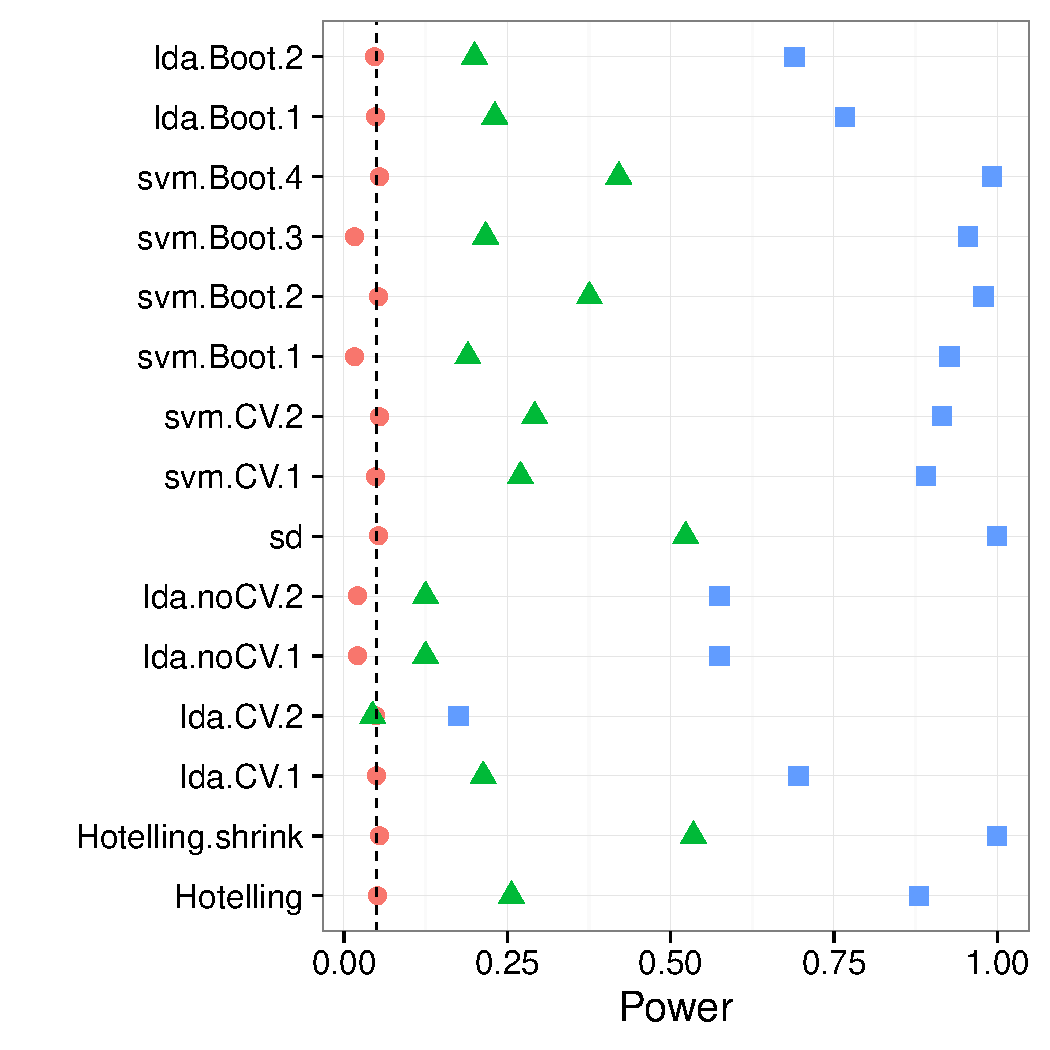
\includegraphics[width=0.7\linewidth]{art/2016-08-30_18_08_08}
	  \caption{
		  \textbf{Bootstrap--}
		  The power of a permutation test with various test statistics. 
		  The power on the $x$ axis. 
		  Effects are color and shape coded. 
		  The various statistics on the $y$ axis. 
		  Their details are given in tables~\ref{tab:collected} and \ref{tab:collected_2}. 
		  Effects vary over $0$ (red circle), $0.25$ (green triangle), and $0.5$ (blue square). 
		  Simulation details in Appendix~\ref{apx:simulation_details}.
		  } 
	\label{fig:bootstrap}
\end{figure}


\subsection{High dimensional classifiers}
\label{sec:highdim}
Inspecting Figure~\ref{fig:simulation_11} (for instance), it can be seen that Hotelling's unregularized  $T^2$ test has similar power as accuracy tests. 
It should thus be argued that the real advantage of the population tests is due to their adaptation to high dimension by regularization, and not only to discretization.
To study this, we call upon several \emph{regularized classifiers}, designed for high dimensional problems. 
In the spirit of the regularized covariance of \emph{Hotelling.shrink}, we try an $l_2$ regularized SVM \citep{REF08a}, and shrinkage based LDA \citep{pang_shrinkage-based_2009,ramey_high-dimensional_2016}. %TODO: verify references
In the spirit of the diagonalized covariance of \emph{sd}, we try a diagonalized LDA \citep{dudoit_comparison_2002}, a.k.a.\ \emph{Gaussian naive Bayes}. 


Simulation results are reported in Figure~\ref{fig:highdim} with naming conventions in Table~\ref{tab:collected_3}.
It can be seen that regularizing a classifier in high dimension, just like a parameter test, improves power. 
It can also be seen that (regularized) parameter tests are still more powerful than (regularized) accuracy tests. 
This was to be expected, since we already saw in (e.g.) Figure~\ref{fig:simulation_11} that the unregularized parameter test, \emph{Hotelling}, is slightly more powerful than unregularized accuracy tests such as (e.g.) \emph{svm.CV.1}.

We can compound the regularization with the bootstrapping from Section~\ref{sec:bootstrap}, to improve finite sample power of the accuracy tests. 
This is done in the \emph{svm.highdim.2} and \emph{lda.highdim.4} tests. 
The latter being one of the very few accuracy tests that achieve the same power as population tests. 
This is exciting news since it shows how to design powerful new high-powered accuracy tests: by sampling test sets with replacement, and by regularizing the classifiers. 


\bigskip

%TODO: change cost in simulation to 0.1
\begin{tcolorbox}
\centering
\begin{tabular}{l|c|c|c|c}
Name & Algorithm & Accuracy & Z-scored & Parameters\\ 
\hline
\hline
svm.highdim.1 & SVM & V-fold & FALSE & cost=10, V=4 \\ 
svm.highdim.2 & SVM & b$0.632$ & FALSE & cost=10, B=50 \\ 
lda.highdim.1 & LDA & V-fold & FALSE & V=4 \\ 
lda.highdim.2 & LDA & V-fold & FALSE & V=4 \\ 
lda.highdim.3 & LDA & V-fold & FALSE & V=4 \\ 
lda.highdim.4 & LDA & b$0.632$ & FALSE & B=50 \\ 
\end{tabular} 
\captionsetup{type=table}
\caption{
The same as Table~\ref{tab:collected} for regularized (high dimensional) predictors. 
\emph{svm.highdim.1} is an $l_2$ regularized SVM \citep{friedman_regularization_2010}. 
\emph{svm.highdim.2} is the same with b$0.632$ instead of V-fold cross validation. 
\emph{lda.highdim.1} is the Diagonal Linear Discriminant Analysis of \cite{dudoit_comparison_2002}.
\emph{lda.highdim.2} is the High-Dimensional Regularized Discriminant Analysis of \cite{ramey_high-dimensional_2016}.
\emph{lda.highdim.3} is the Shrinkage-based Diagonal Linear Discriminant Analysis of \cite{pang_shrinkage-based_2009}.
\emph{lda.highdim.4} is the same with b$0.632$.
} 
\label{tab:collected_3}
\end{tcolorbox}


\begin{figure}[ht]
\centering
	  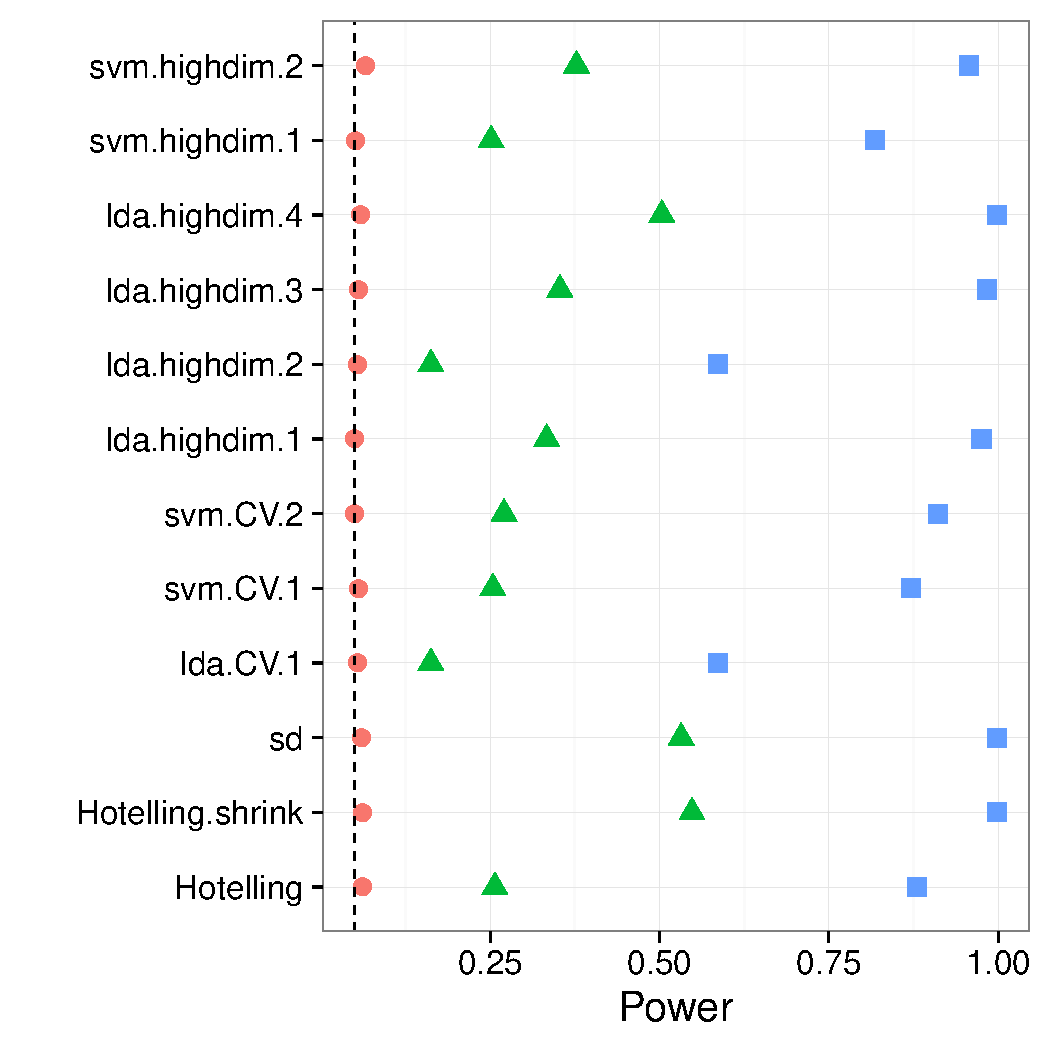
\includegraphics[width=0.7\linewidth]{art/2016-08-17_08_48_18}
	  \caption{
\textbf{HighDim Classifier--} 
		The power of a permutation test with various test statistics. 
		The power on the $x$ axis. 
		Effects are color and shape coded. 
		The various statistics on the $y$ axis. 
		Their details are given in tables~\ref{tab:collected} and \ref{tab:collected_3}. 
		Effects vary over $0$ (red circle), $0.25$ (green triangle), and $0.5$ (blue square). 
		Simulation details in Appendix~\ref{apx:simulation_details}.
} 
	\label{fig:highdim}
\end{figure}





\subsection{A good accuracy test}
For the cases a population test cannot replace an accuracy test, we collect some conclusions and best practices.

\paragraph{Sample size.} The conservativeness of accuracy tests decrease with sample size. 


\paragraph{Regularize.}
Regularization proves crucial to detection power in low signal to noise regimes: in high dimension and\slash or in the presence of strong correlations. 
We find that the Shrinkage-based Diagonal Linear Discriminant Analysis of \cite{pang_shrinkage-based_2009} is a particularly good performer, but more research is required on this matter. 
We also conjecture that the power-maximizing regularization is larger than the error-minimizing regularization.

\paragraph{Smooth accuracy.}
Smooth accuracy estimate by cross validating with replacement. The bLOO estimator, in particular, is preferable over V-fold.

\paragraph{Permute features.} Permuting features, such as in \cite{golland_permutation_2005}, is easier than permuting labels. 
It allows to preserve the balance of folds after a permutation, without refolding.

\paragraph{Resubstitution accuracy in low dimension.} Resubstitution accuracy is useful in low SNR regimes, such as low dimensional problems, because it avoids cross validation without compromising power. 
In high dimension, the power loss is considerable compared to a cross validated approach. 
We attribute this to the compounding of discretization and concentration effects: the difference between the sampling distribution of the resubstitution accuracy is simply indistinguishable under the null and under the alternative. 
In low dimensional problems, the discretization is less impactful, and the computational burden of cross validation can be avoided by using the resubstitution accuracy. 
There is a fundamental difference between V-folding and resubstitution. The latter should not be thought of as the limit of the former. 
 

\paragraph{Don't z-score.} There is no gain in z-scoring the accuracy scores. Our motivating rational was clearly flawed. %TODO: why?

















\subsection{Related Literature}
\cite{ojala_permutation_2010} study the power of two accuracy tests differing in the permutation scheme:
One testing the ``no signal'' null hypothesis, and the other testing the ``independent features'' null hypothesis. 
They perform an asymptotic analysis, and a simulation study. 
They also apply various classifiers to various data sets. 
Their emphasis is the effect of the underlying classifier on the power, and the potential of the ``independent features'' test for feature selection.
This is a very different emphasis from our own.


\cite{olivetti_induction_2012} and \cite{olivetti_statistical_2014} looked into the problem of choosing a good accuracy test. 
They propose a new test they call an \emph{independence test}, and demonstrate by simulation that it has more power than other accuracy tests, and can deal with non-balanced data sets. 
We did not include this test in the battery we compared, but we note the following: 
(a) The independence test of \cite{olivetti_induction_2012} relies on a discrete test statistic. 
It may probably be improved with the methods discussed in this section, before the application of \cite{olivetti_induction_2012}'s independence test. 
(b) In contrast with the underlying motivation of \cite{olivetti_induction_2012}'s independence test, we did not find that balancing the data folds affects the power of the test. 


\cite{golland_permutation_2003} and \cite{golland_permutation_2005} study accuracy tests using simulation, neuroimaging data, genetic data, and analytically.
Their analytic results formalize our intuition from Section~\ref{sec:introduction} on the effect of concentration of the accuracy statistic:
The finite Vapnik–Chervonenkis dimension requirement \citep[Sec 4.3]{golland_permutation_2005} prevents the permutation p-value from (asymptotically) concentrating near $1$. 
Like ourselves, they also find that the power increases with the size of the test set. 
This is seen in Fig.4 of \citet{golland_permutation_2005}, where the size of the test-set, $K$, governs the discretization. 
Since they permute features, not labels, then all their permutation samples are balanced, and there is no issue of refolding. 

\cite{golland_permutation_2005} simulate the power of accuracy tests by sampling from a Gaussian mixture family of models, and not from a location family as our own simulations. 
Under their model 
$$(x_i|y_i=1) \sim p \gauss{\mu_1,I}+ (1-p) \gauss{\mu_2,I}$$ 
and 
$$(x_i|y_i=-1) \sim (1-p) \gauss{\mu_1,I}+ p \gauss{\mu_2,I}.$$
Varying $p$ interpolates between the null distribution $(p=0.5)$ and a location shift model $(p=0)$. 
We now perform the same simulation as \cite{golland_permutation_2005}, after parameterizing $p$ so that $p=0$ corresponds to the null model, and in the same dimensionality as our previous simulations
We find that also in this mixture class of models a population test has more power than an accuracy test (Figure~\ref{fig:golland}).



\begin{figure}[ht]
\centering
	  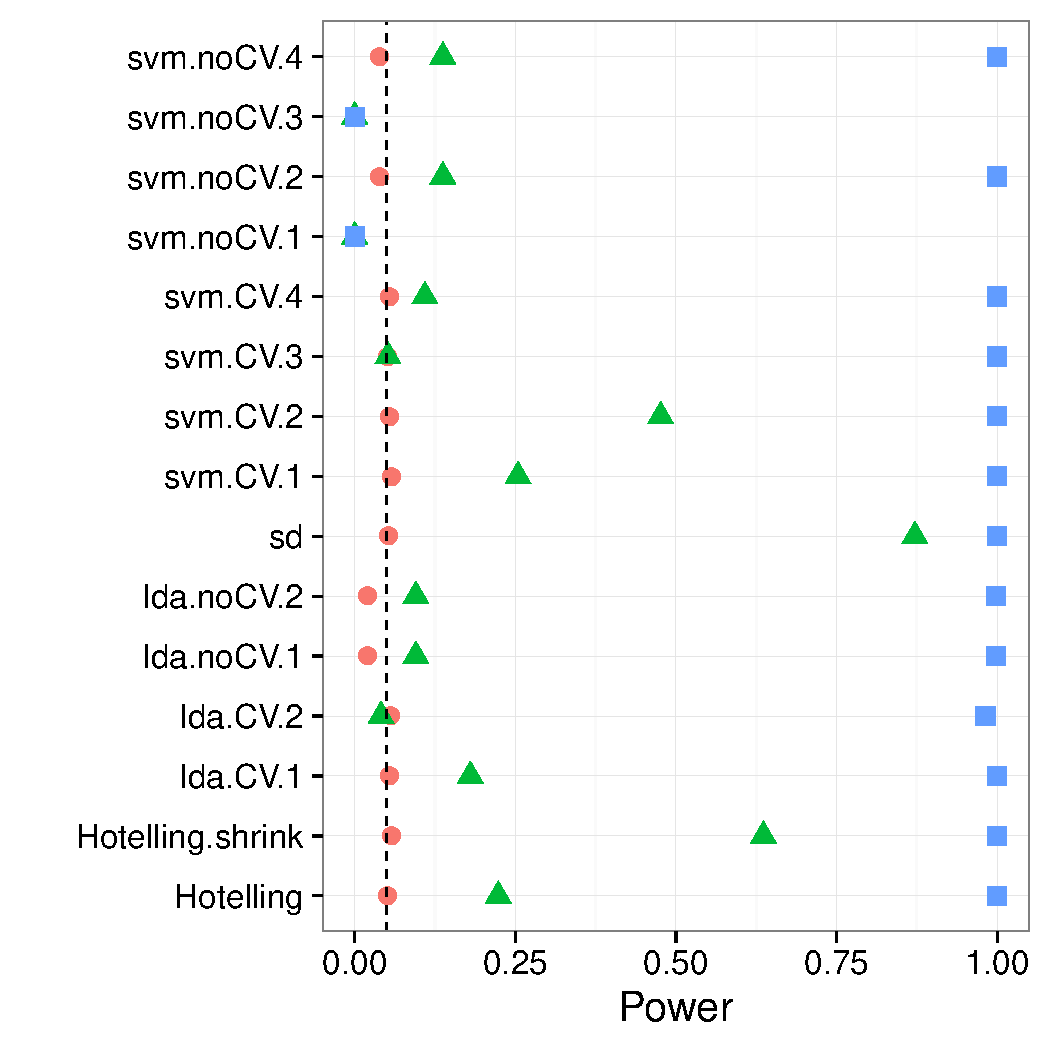
\includegraphics[width=0.7\linewidth]{art/2016-08-08_07_33_05}
	  \caption{\textbf{Mixture--} $\x_i = \chi_i \mu + \eta_i; \chi_i = \set{-1,1}$ and $\prob{\chi_i=1}=(1/2-p)^{\y^*_i}  (1/2+p)^{1-\y^*_i}$. $\mu$ is a $p$-vector with $3/\sqrt{p}$ in all coordinates.
	  The effect, $p$, is color and shape coded and varies over $0$ (red circle), $1/4$ (green triangle) and $1/2$ (blue square). }
	\label{fig:golland}
\end{figure}










\subsection{Epilogue}
Given all the above, we find the popularity of accuracy tests for signal detection quite puzzling. 
We believe this is due to a reversal of the inference cascade. 
Researchers first fit a classifier, and then ask if the classes are any different.
Were they to start by asking if classes are any different, and only then try to classify, then population tests would naturally arise as the preferred method. 
As put by \cite{ramdas_classification_2016}:
\begin{quote}
The recent popularity of machine learning has resulted in the extensive teaching and use
of prediction in theoretical and applied communities and the relative lack of awareness or
popularity of the topic of Neyman-Pearson style hypothesis testing in the computer science
and related ``data science'' communities.
\end{quote}






%\section{Acknowledgments}
%TODO
% isf 900/60, Jelle, Jesse B.A. Hemerik, Yakir Brechenko, Omer Shamir, Joshua Vogelstein, Gilles Blanchard, Jason 




\newpage
\bibliographystyle{abbrvnat}
\bibliography{permuting_accuracy.bib}

\appendix





\newpage
%%%%%%%%%%%%%%%%%%%%%%%%%%%%%%%%%%%%%%%%%%%%%%%%%%%%%%%%
%\section{Analysis pipeline}
%\label{apx:analysis}
%
%Here is the analysis pipeline of \cite{stelzer_statistical_2013} we for the auditory data in \cite{gilron_quantifying_2016}.
%Denoting by 
%$i=1,\dots,I$ the subject index, 
%$v=1,\dots,V$ the voxel index, and 
%$s = 1,\dots,S$ the permutation index. 
%Since regions\footnote{\emph{searchlight} or \emph{sphere} in the MVPA parlance} are centered around a unique voxel, the voxel index $v$ also serves as a unique region index.
%Algorithm~\ref{algo:statistic} computes a region-wise test statistic, which is compared to its permutation null distribution computed by Algorithm~\ref{algo:permutation}.
%
%
%\begin{algorithm}[H]
%\caption{Compute a group parametric map.}
%\label{algo:statistic}
%
% \KwData{fMRI scans, and experimental design.}
% \KwResult{Brain map of group statistics: $\{\bar{T}_v\}_{v=1}^V$}
%	 \For{$v \in 1,\dots,V$}{
%		 \For{$i \in 1,\dots,I$}{
%			 $T_{i,v} \leftarrow$ test statistic for subject $i$ in a region centered at $v$.
%			 } 	  
%	  	 $\bar{T}_{v} \leftarrow \frac{1}{I}\sum_{i=1}^I T_{i,v}$. 
% 	 }
%\end{algorithm}
%
%
%\begin{algorithm}[H]
%\caption{Compute a permutation p-value map.} 
%\label{algo:permutation}
%
% \KwData{fMRI scans of $20$ subjects, experimental design.}
% \KwResult{Brain map of permutation p-values: $\{p_v\}_{v=1}^V$}
%  \For{$s \in 1,\dots\,S$}{
%    	    permute labels\;
%    	    $\bar{T}_{v}^s \leftarrow$ parametric map 
%  
%  	}
%\end{algorithm}
%
%





\newpage
%%%%%%%%%%%%%%%%%%%%%%%%%%%%%%%%%%%%%%%%%%%%%%%%%%%%%%%%%%%%%%%%%%55
\section{Simulation Details}
\label{apx:simulation_details}

The following details are common to all the reported simulations, unless stated otherwise in a figure's caption. 
The \R code for the simulations can be found in [TODO].

Each simulation is based on $4,000$ replications. 
In each replication, we generate $n$ i.i.d. samples from a shift model $\x_i = \mu \y^*_i + \eta_i$.
Where $y^*_i=\set{0,1}$ is the class of subject $i$ in dummy coding. 
Recalling that $y_i=\set{-1,1}$ is the class in effect coding, then clearly $y_i=2 y^*_i-1$.
The noise is distributed as $\eta_i \sim \gaussp{p}{0,\Sigma}$. 
The sample size $n=40$. 
The dimension of the data is $p=23$. 
The covariance $\Sigma=I$. 
Effects, i.e. shifts $\mu$, are equal coordinate $p$-vectors with coordinates that vary over $\mu \in \set{0,1/4,1/2}$.

Having generated the data, we compute each of the test statistics in Table~\ref{tab:collected}.
For test statistics that require data folding, we used $8$ folds. 
We then compute a permutation p-value by permuting the class labels, and recomputing each test statistic. 
We perform $400$ such permutations. 
We then reject the $\mu_i=0$ null hypothesis if the permutation p-value is smaller than $0.05$.
The reported power is the proportion of replication where the permutation p-value falls below $0.05$.




\newpage
%%%%%%%%%%%%%%%%%%%%%%%%%%%%%%%%%%%%%%%%%%
\section{Simulation Results}
\label{apx:simulations}




\begin{figure}[h]
	\centering
	\caption{
		The power of a permutation test with various test statistics. 
		The power on the $x$ axis. 
		Effects are color and shape coded. 
		The various statistics on the $y$ axis. 
		Their details are given in Table~\ref{tab:collected}. 
		Effects vary over $0$ (red circle), $0.25$ (green triangle), and $0.5$ (blue square). 
		Simulation details in Appendix~\ref{apx:simulation_details}.
		Cross-validation was performed with balanced and unbalanced data folding. See sub-captions.}	
	\label{fig:simulation_1}
	\begin{subfigure}{.5\textwidth}
		\centering
		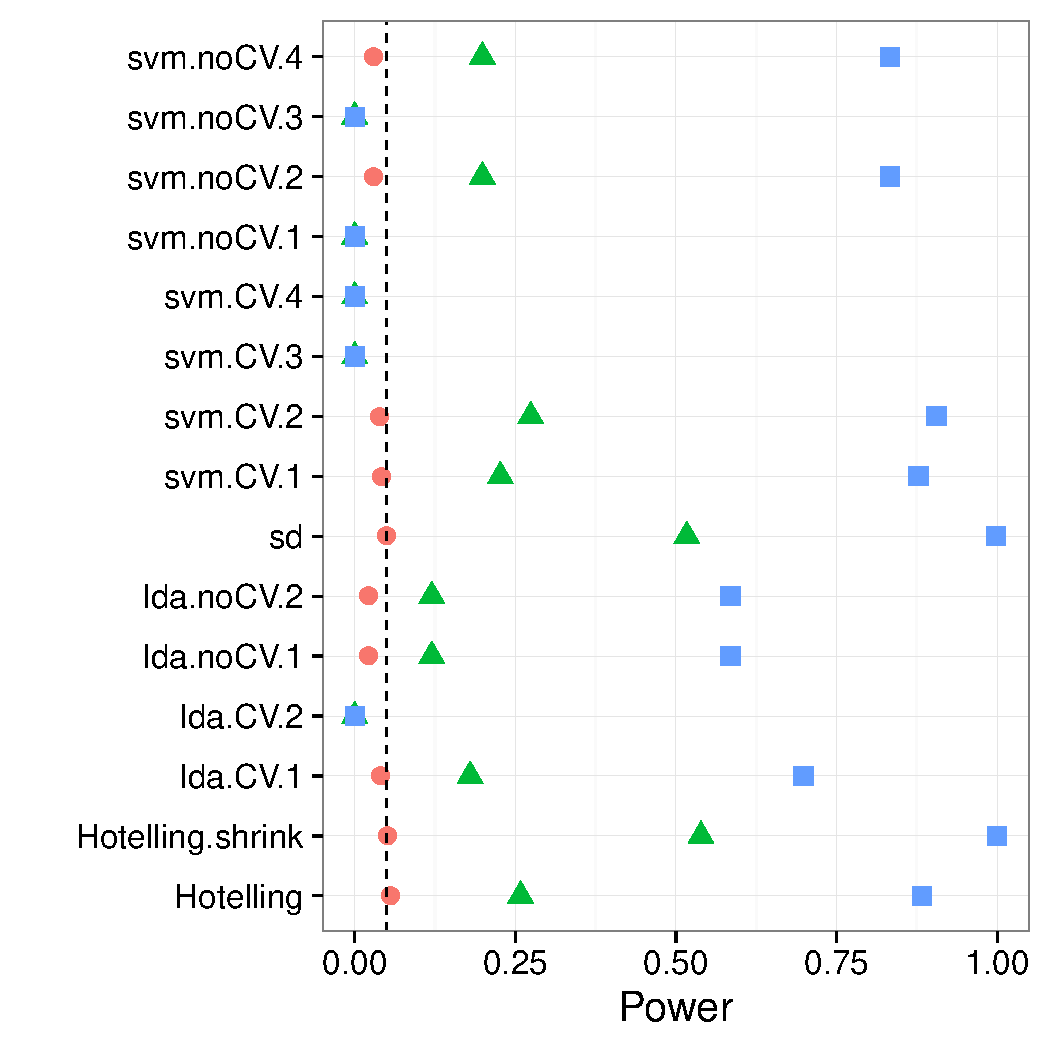
\includegraphics[width=1\linewidth]{art/2016-07-26_20_55_48}
		\caption{\textbf{Unbalanced.}} %TODO: caption  
		\label{fig:simulation_11}
	\end{subfigure}%
	\begin{subfigure}{.5\textwidth}
		\centering
		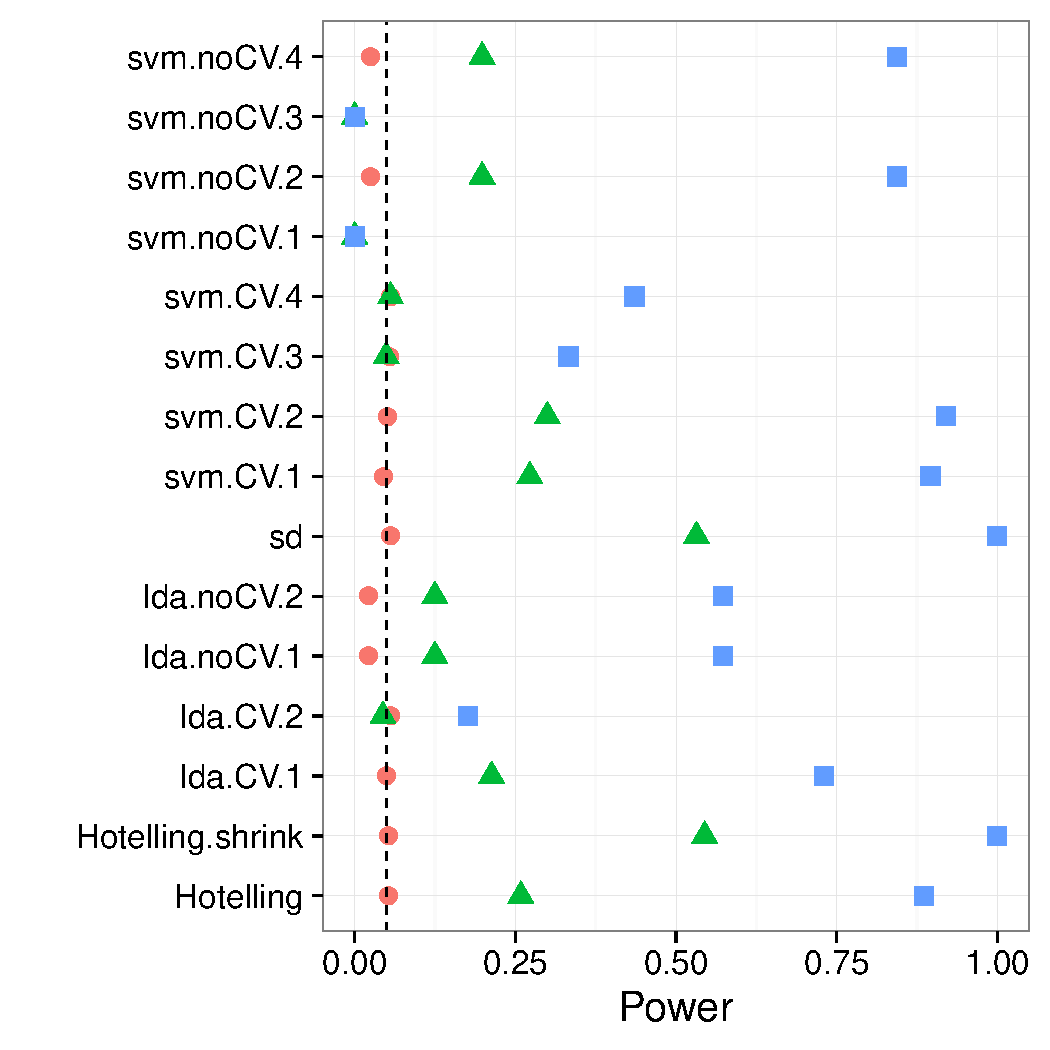
\includegraphics[width=1\linewidth]{art/2016-07-27_11_42_05}
		\caption{\textbf{Balanced.}} %TODO: caption 
		\label{fig:simulation_12}
	\end{subfigure}
\end{figure}





\begin{figure}[h]
\centering
\caption{\mycaption}	
\label{fig:n_folds}
	\begin{subfigure}{.5\textwidth}
	  \centering
	  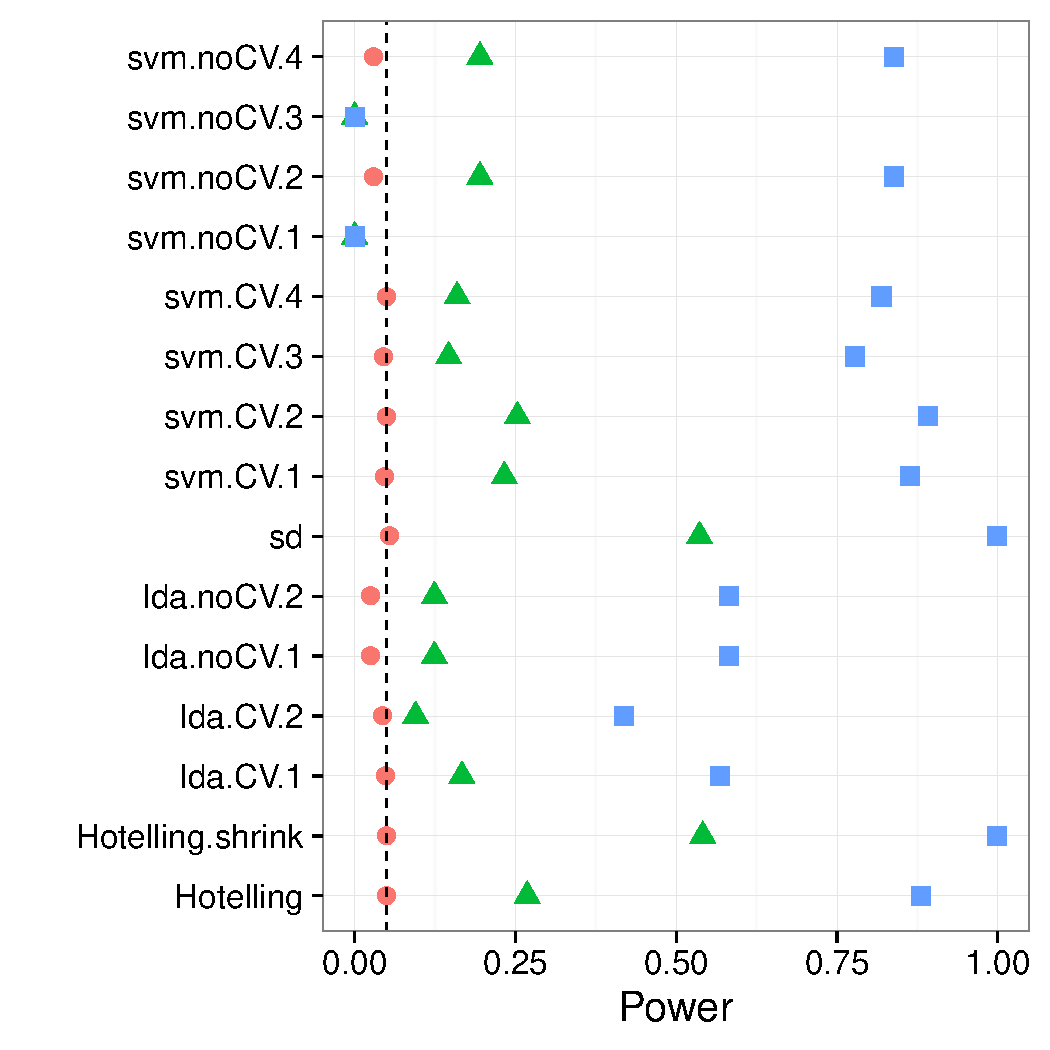
\includegraphics[width=1\linewidth]{art/2016-07-27_21_21_12}
	  \caption{\textbf{2-fold} cross validation. Balanced folding.}  
	\label{fig:n_folds_1}
	\end{subfigure}%
	\begin{subfigure}{.5\textwidth}
	  \centering
	  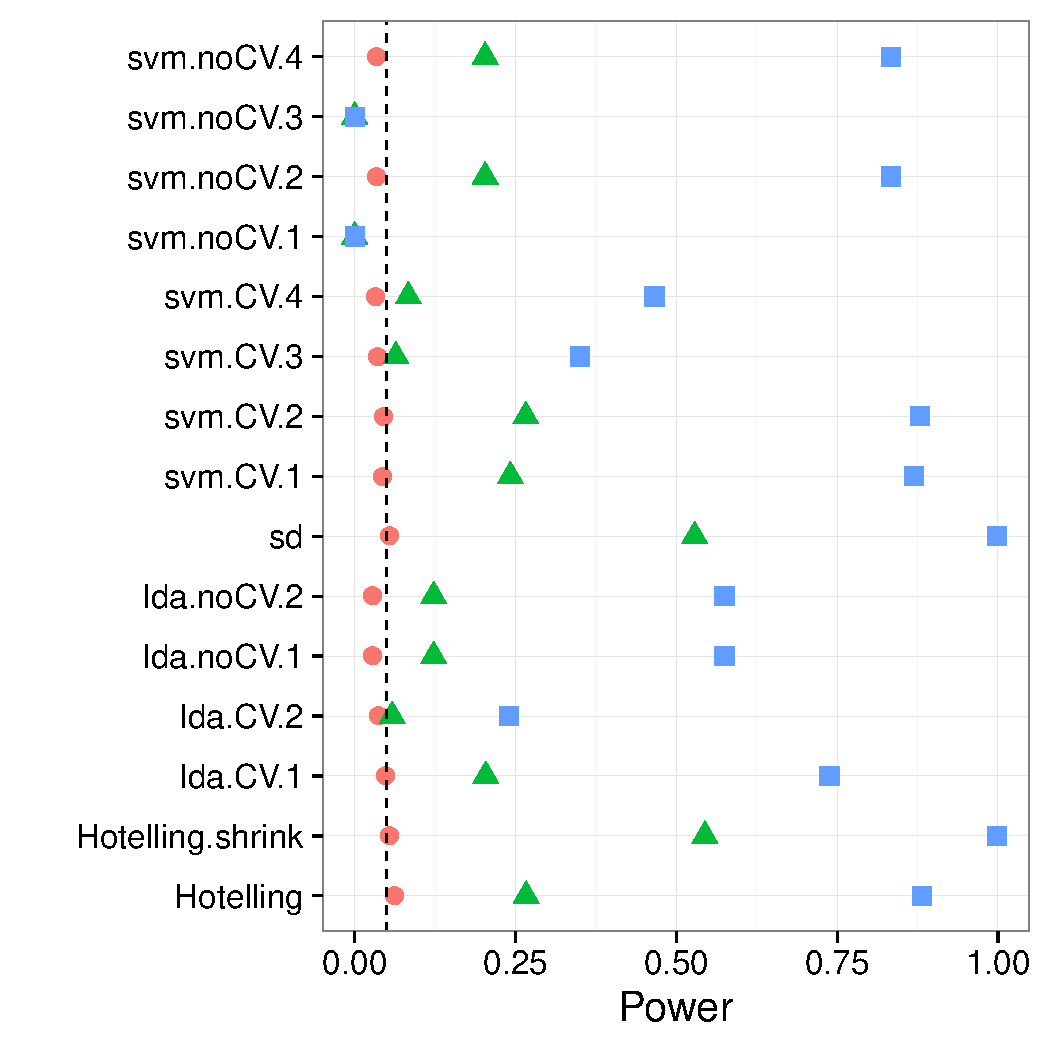
\includegraphics[width=1\linewidth]{art/2016-07-29_07_18_24}
	  \caption{\textbf{20-fold} cross validation. Balanced folding} 
	\label{fig:n_folds_2}
	\end{subfigure}
\end{figure}



\begin{figure}[h]
\centering
\caption{\mycaption}	
\label{fig:n_folds_unbalanced}
	\begin{subfigure}{.5\textwidth}
	  \centering
	  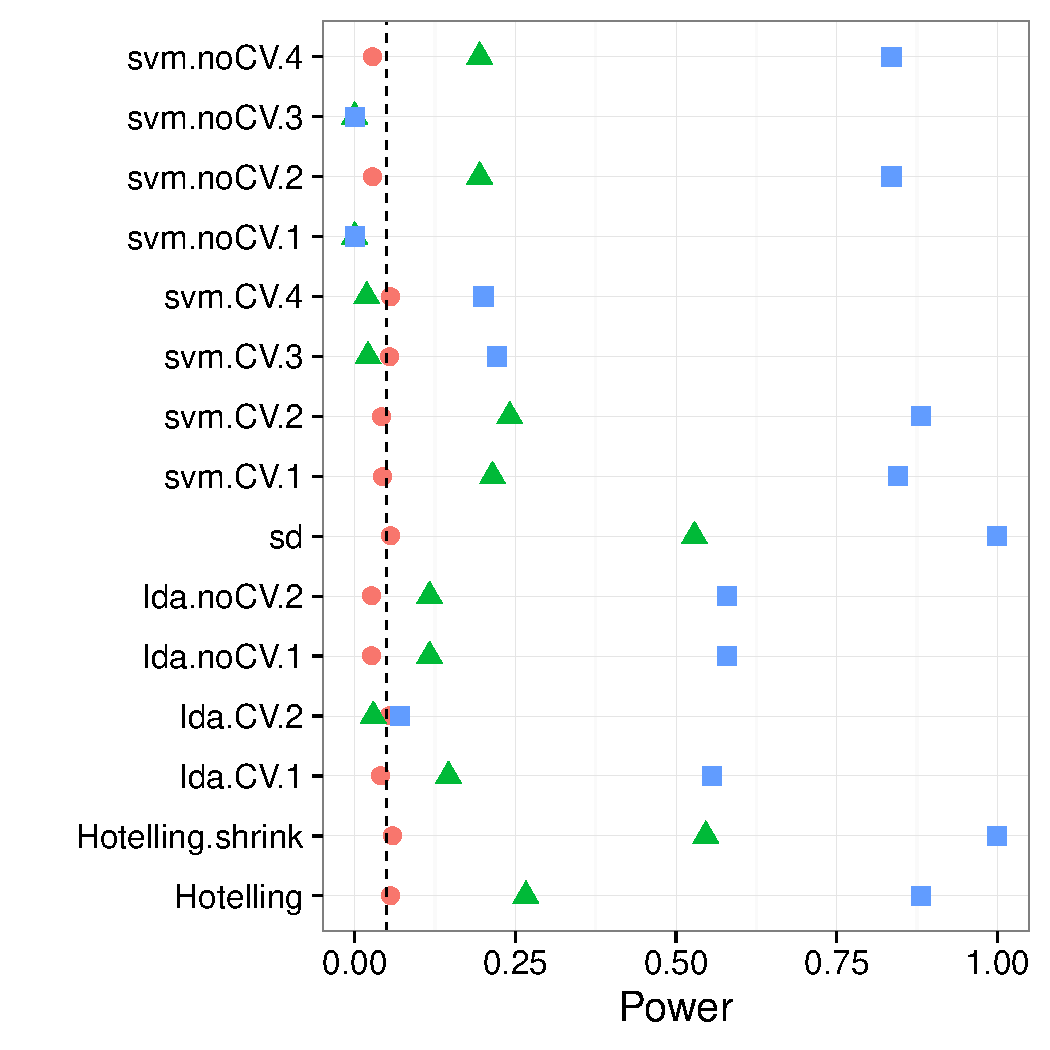
\includegraphics[width=1\linewidth]{art/2016-08-05_09_37_35}
	  \caption{\textbf{2-fold} cross validation. Unbalanced folding.} 
	\label{fig:n_folds_unbalanced_1}
	\end{subfigure}%
	\begin{subfigure}{.5\textwidth}
	  \centering
	  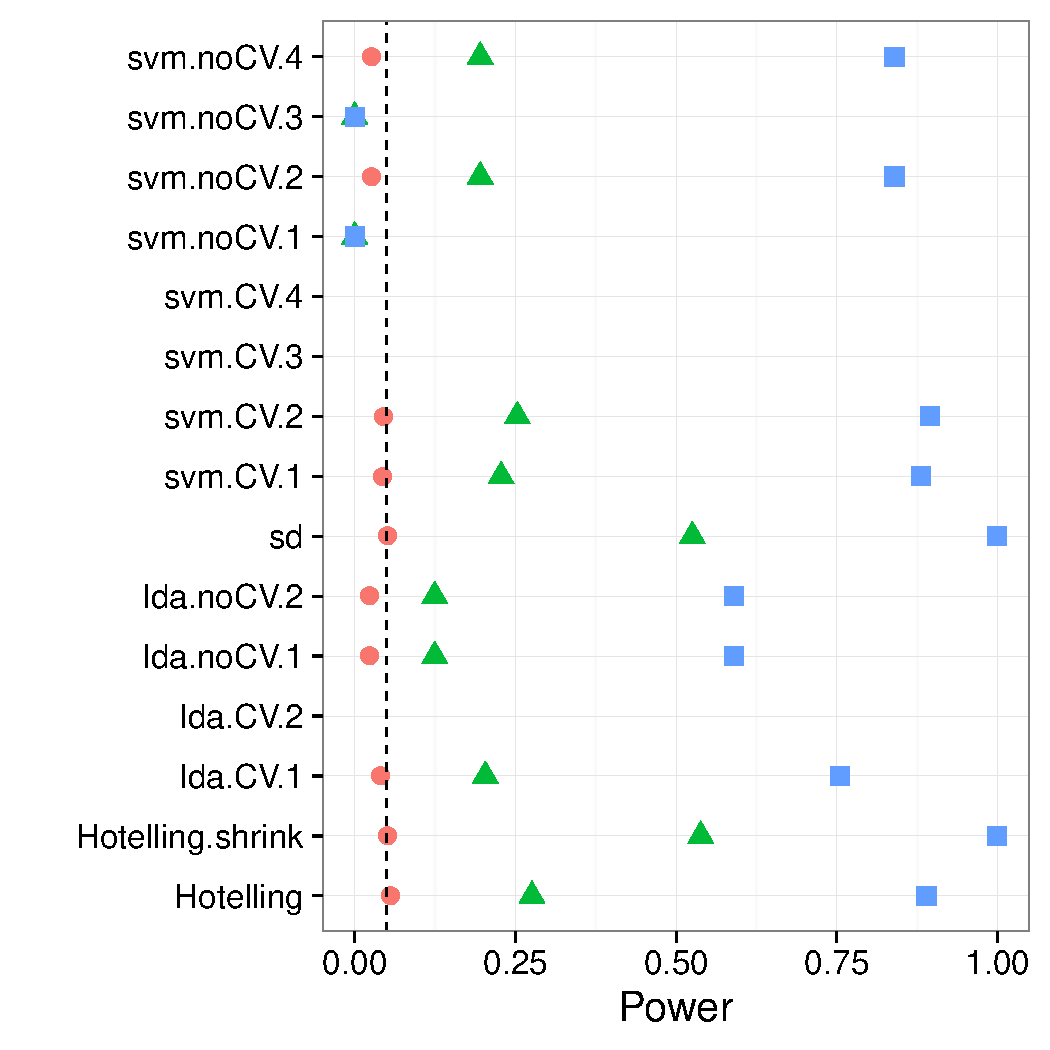
\includegraphics[width=1\linewidth]{art/2016-08-06_07_57_22}
	  \caption{\textbf{20-fold} cross validation. Unbalanced folding.} 
	\label{fig:n_folds_unbalanced_2}
	\end{subfigure}
\end{figure}



\begin{figure}[h]
\centering
\caption{\mycaption}	
%\label{fig:simulation_1}
	\begin{subfigure}{.5\textwidth}
	  \centering
	  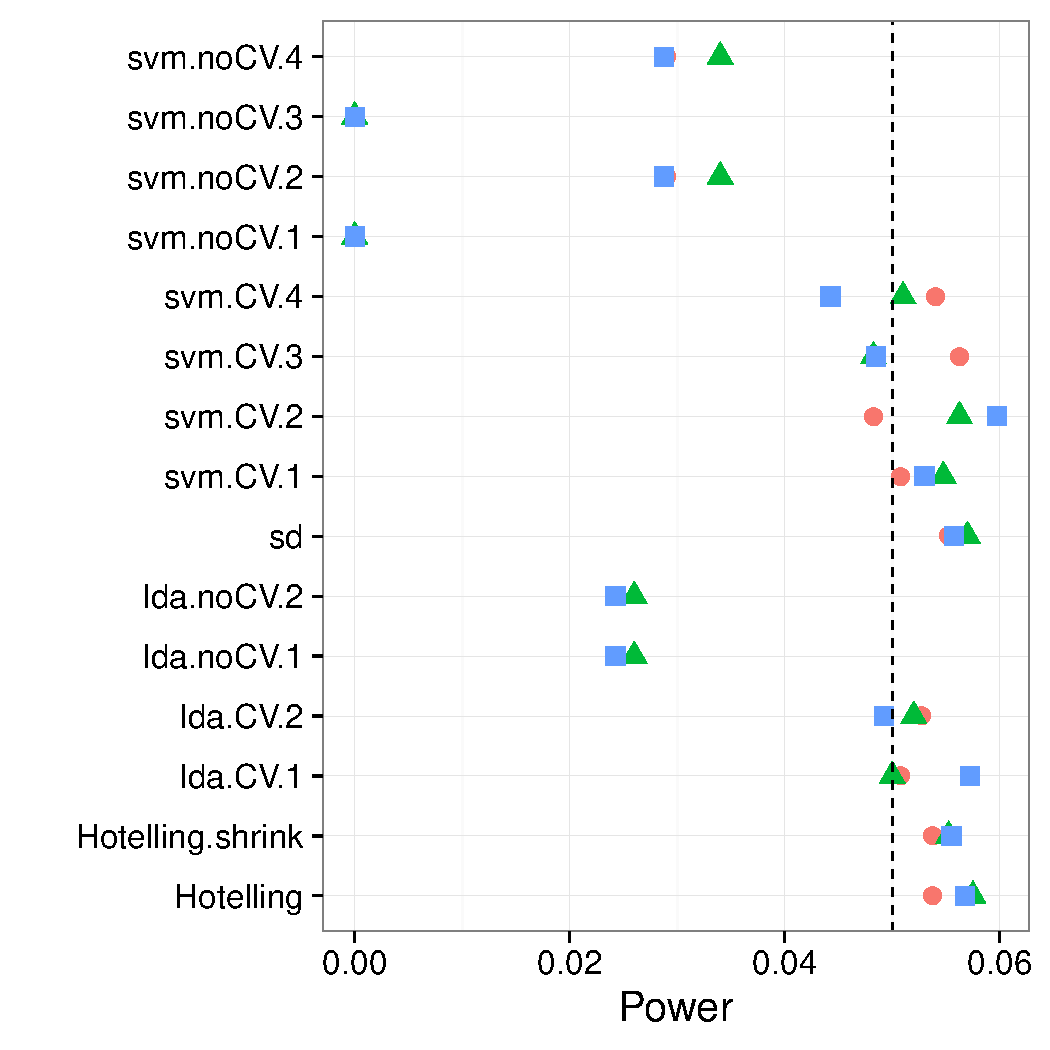
\includegraphics[width=1\linewidth]{art/2016-07-30_10_33_05}
	  \caption{\textbf{Scale Change--} $\x_i =  \eta_i * \mu^ {\y^*_i}$ so that the effects are a scale change.}  
	\label{fig:scale_change}
	\end{subfigure}%
	\begin{subfigure}{.5\textwidth}
	  \centering
	  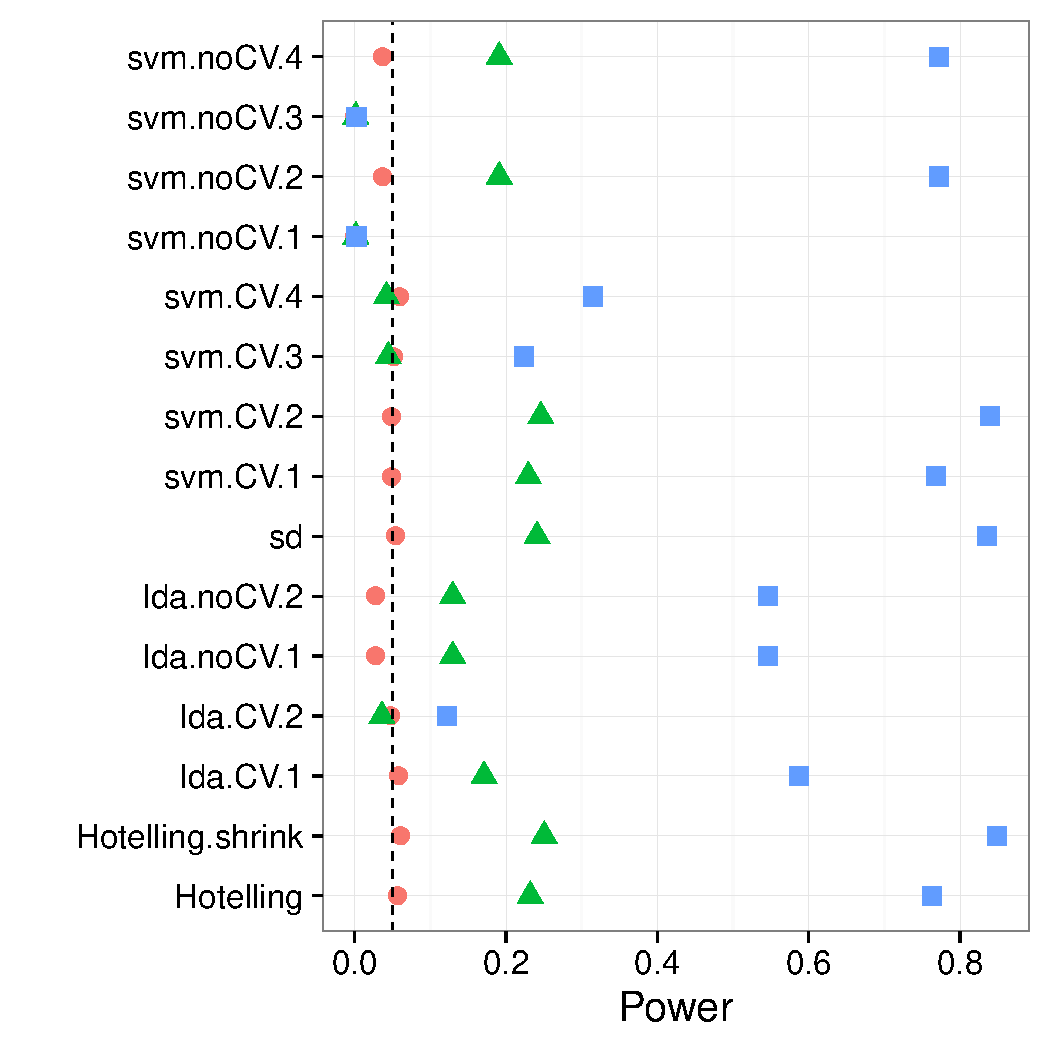
\includegraphics[width=1\linewidth]{art/2016-08-04_19_32_17}
	  \caption{\textbf{Heavytailed--} $\eta_i$ is not $p$-variate Gaussian, but rather $p$-variate t, with $df=3$ .  } 
	\label{fig:t_null}
	\end{subfigure}
\end{figure}




\begin{figure}[h]
\centering
\caption{\mycaption}	
\label{fig:large_sample}
	\begin{subfigure}{.5\textwidth}
	  \centering
	  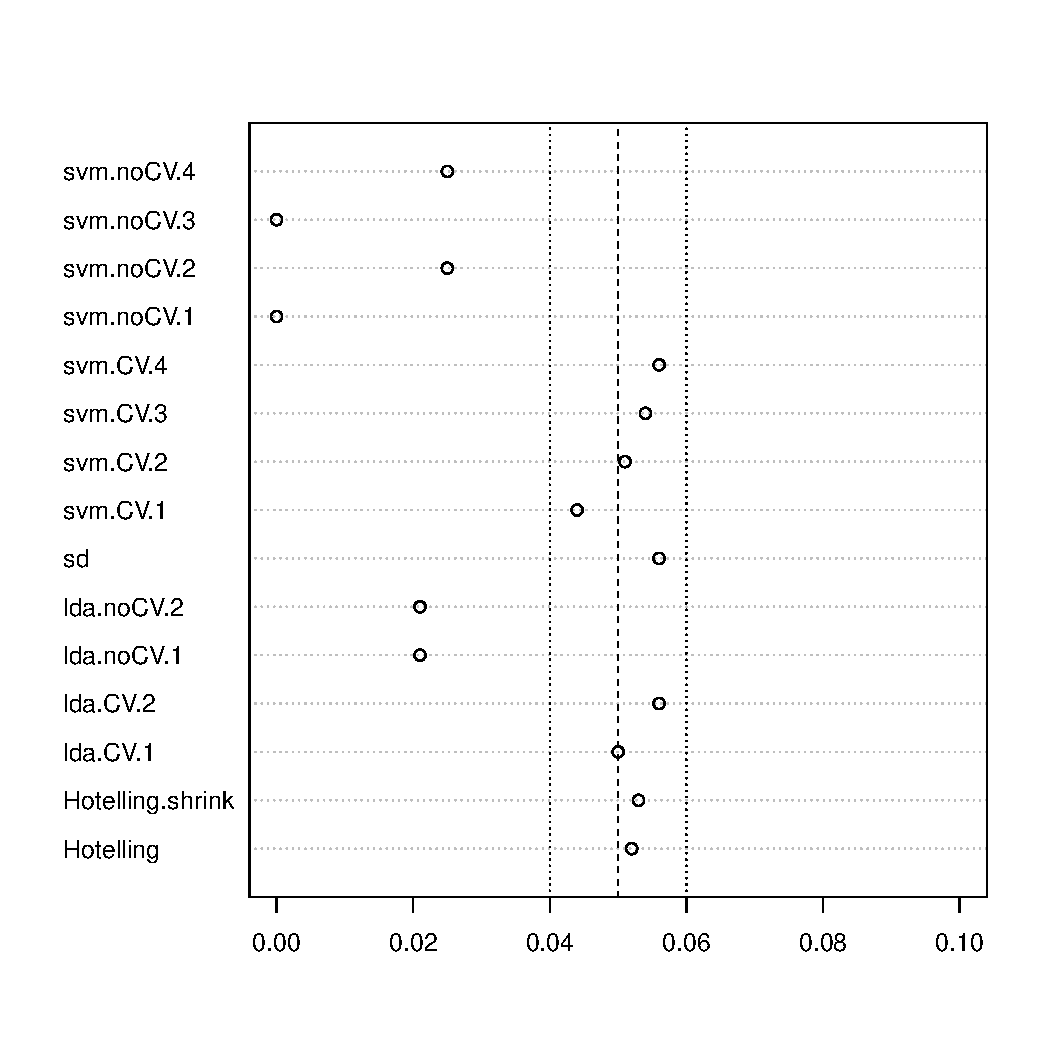
\includegraphics[width=1\linewidth]{art/2016-07-27_11_42_05zoom}
	  \caption{\textbf{Low-Dimension--} False positive rates for $n=40$.} 
	\label{fig:large_sample_1}
	\end{subfigure}%
	\begin{subfigure}{.5\textwidth}
	  \centering
	  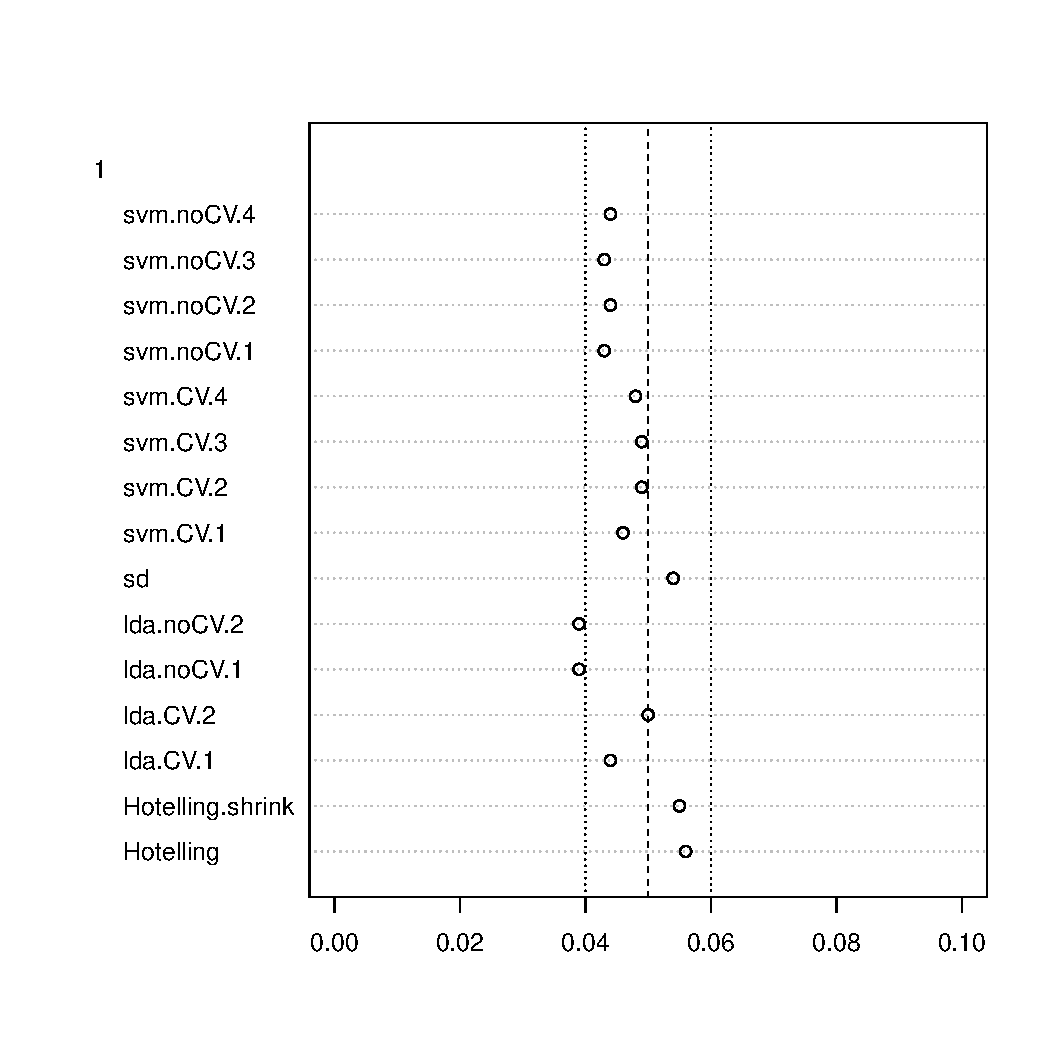
\includegraphics[width=1\linewidth]{art/2016-08-04_13_59_33zoom}
	  \caption{\textbf{High-Dimension--} False positive rates for $n=400$.} 
	\label{fig:large_sample_2}
	\end{subfigure}
\end{figure}




\begin{figure}[h]
\centering
\caption{\mycaption}	
	\begin{subfigure}{.4\textwidth}
	  \centering
	  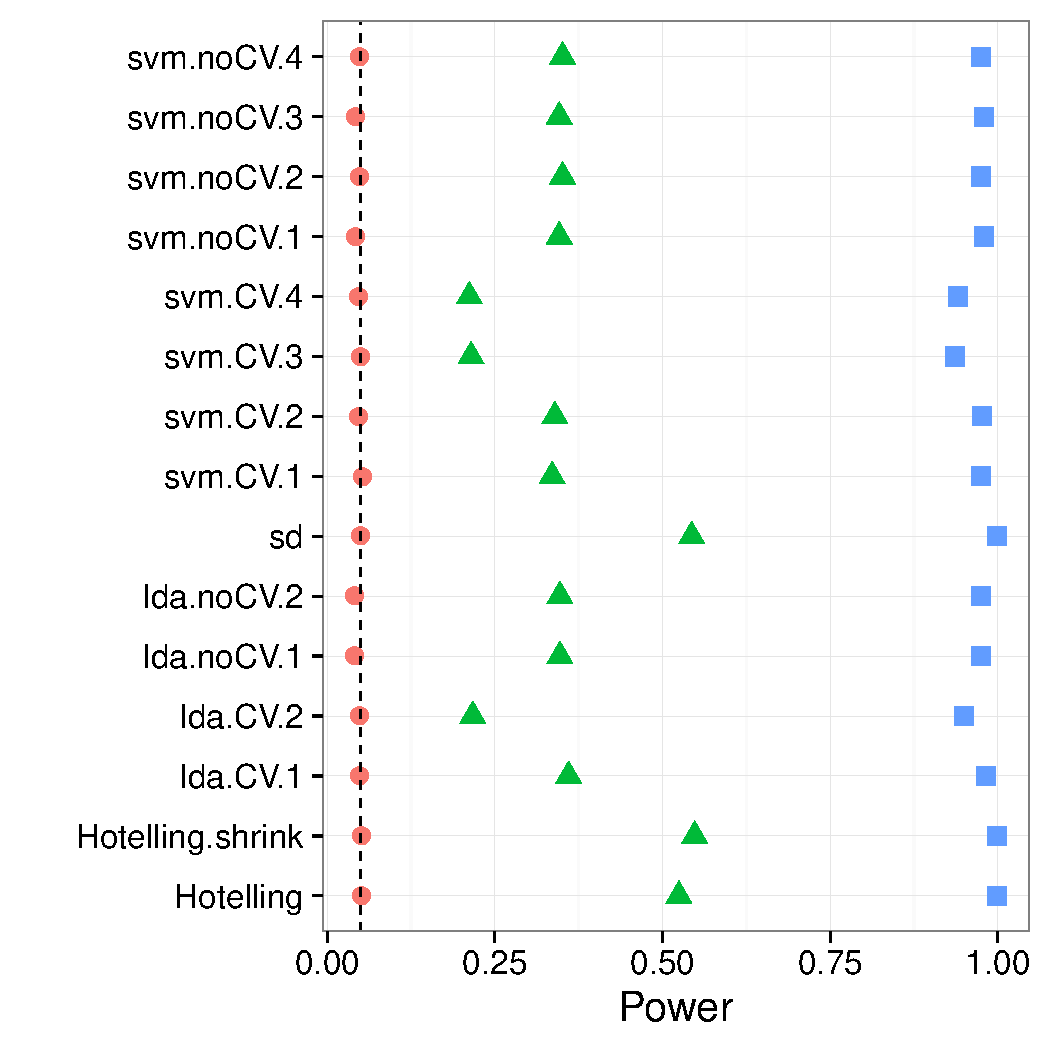
\includegraphics[width=1\linewidth]{art/2016-08-11_08_32_39}
	  \caption{\textbf{High-Dimension, local alternative--} $n=400$, $\mu \in \frac{1}{\sqrt{10}} \times \set{0,1/4,1/2}.$} 
	\label{fig:large_sample_3}
	\end{subfigure}
		\begin{subfigure}{.4\textwidth}
		  \centering
		  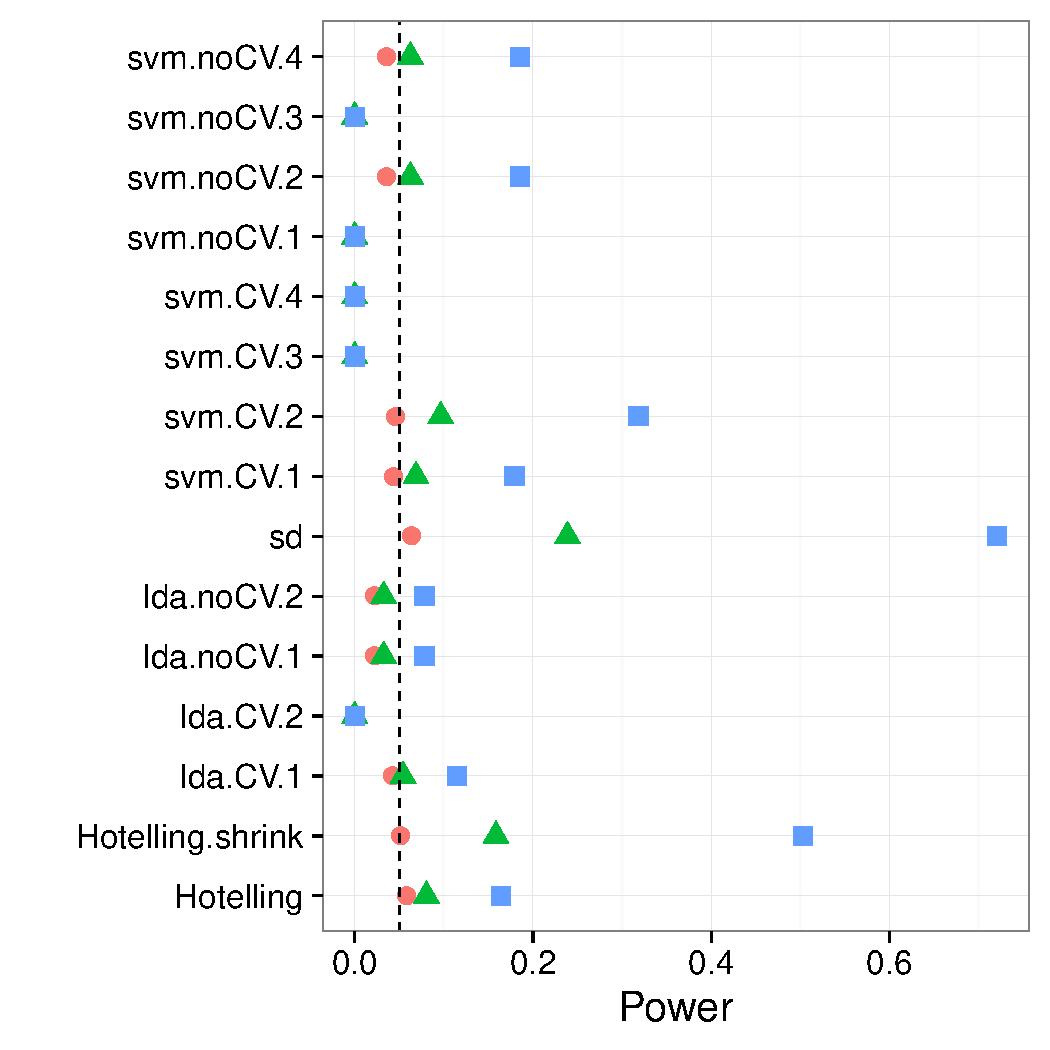
\includegraphics[width=1\linewidth]{art/2016-08-07_20_11_46}
		  \caption{\textbf{AR(1) dependence--} $\Sigma_{k,l}=\rho^{|k-l|}; \rho=0.8$. } 
		\label{fig:ar_1}
	\end{subfigure}
\end{figure}




\end{document}
